\documentclass[11pt,a4paper]{article}
\title{TfW: Preliminary results for the Class 150 design}
\usepackage{cite}
\usepackage{hyperref}
\usepackage{textcomp}
\usepackage{amssymb}
\usepackage{subcaption}
\usepackage{amsfonts}
\newcommand{\norm}[1]{\left\lVert#1\right\rVert}
\usepackage[left=2cm,right=2cm,top=2cm,bottom=3cm]{geometry}
\usepackage{amsmath}
\setlength\parindent{0pt}
\usepackage{float}
\usepackage{placeins}
\pretolerance=10000
\tolerance=2000
\emergencystretch=10pt
\author{Lucy Henley, Joshua Moore, Timothy Ostler \& Thomas Woolley\footnote{moorej16@cardiff.ac.uk, henleyl1@cardiff.ac.uk, ostlert@cardiff.ac.uk,woolleyt1@cardiff.ac.uk}}
\usepackage{graphicx}
\graphicspath{{./matlab_and_plots/}}
\begin{document}
\maketitle

\section*{Key points}
\begin{itemize}
\item We have integrated the seat layout of both carriages of the Class 150 into our software from the designs provided.
\item We achieved a maximum seat occupancy of $22.5\%$, whilst strictly adhering to a $2$m social distancing measure. 
\item Preliminary stochastic simulations suggest our solutions are optimal.
\item We have developed a web-based application for the Class 150 train seating that allows the user to specify the social distancing measure and return the maximal capacity. Available here: \href{https://lucyhenley.shinyapps.io/TFW_socialdistancing/}{https://lucyhenley.shinyapps.io/TFW\_ socialdistancing/}
\item We provide a user-friendly theoretical framework to produce optimal seating arrangements while adapting to dynamic social distancing measures.
\end{itemize}

\section*{What we could do next}
\begin{itemize}
\item Carry out the computations for all other train designs, and integrate these designs into the web-application for TfW use.
\item Include passenger direction to the analysis; a 1m social distance may be sufficient for passengers facing away from each other.
\item Include the use of plastic shields for each carriage type in computation, allowing for possible cost-benefit analysis.
\item Develop computational techniques to seek more optimal seating arrangements.
\end{itemize}



\section*{Methods and results}
Following our discussions, we added the seating arrangements for the Class 150 train layout to our software. Distance calculations are taken from the centre point of each seat, upon selecting a fixed seat, the algorithm sweeps through all other seats and removes any seat that in within the social distance measure provided, repeating this process until all available seats have a checked. In order to find an optimal solution, we simulated the seat selection randomly 10,000 times for each carriage (see \autoref{fig:Stochastic_sims}), we then selected the order of fixed seats that yielded the greatest capacity. The results of the optimal seat selection algorithm are displayed in Figure \ref{Demonstration_pics} and in Table \ref{tab:performance}. 



\begin{figure}[H]
         \centering
 \begin{subfigure}[b]{0.48\textwidth}
         \centering
         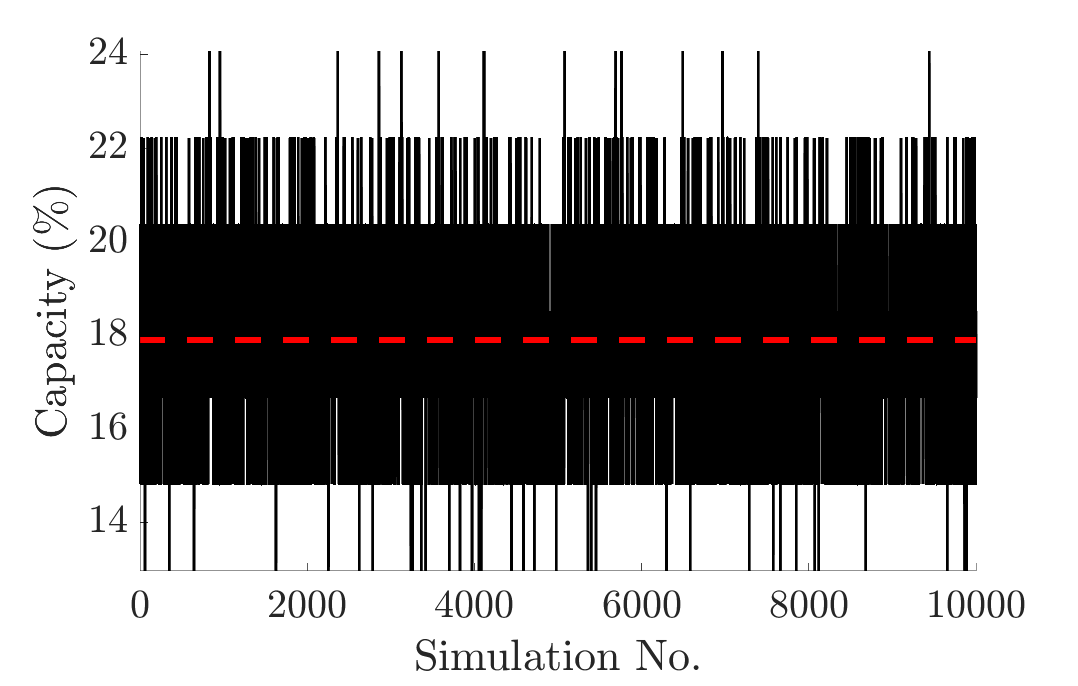
\includegraphics[width=1\textwidth]{tfw_car1_sim_plot_write.png}
         \caption{Stochastic seat seat selection results for carriage 1.}
         \label{fig:sim1}
     \end{subfigure}
          \hfill
     \begin{subfigure}[b]{0.48\textwidth}
         \centering
         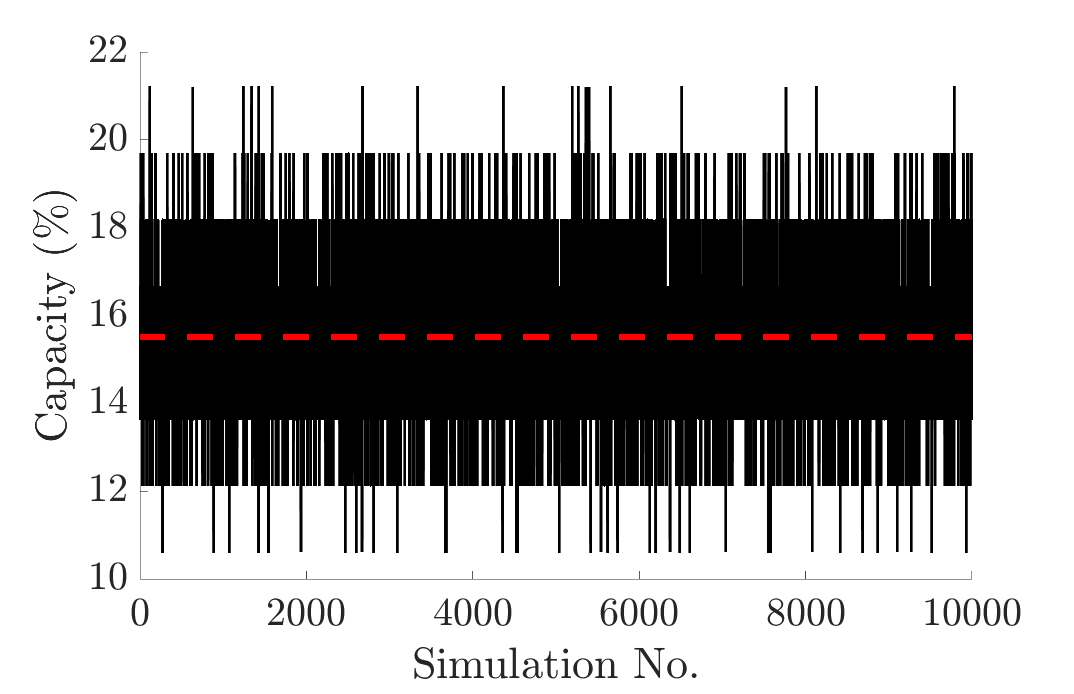
\includegraphics[width=1\textwidth]{tfw_car2_sim_plot_write.png}
         \caption{Stochastic seat seat selection results for carriage 2.}
         \label{fig:sim2}
     \end{subfigure}
     
 
 \caption{Results from stochastic seat selections. The fixed seats where selected at random, the algorithm then swept through all seats and removed seats that were too close. The black line represents the resulting capacity from each simulation, while the dashed red line corresponds to the mean of all simulations.}
        \label{fig:Stochastic_sims}
\end{figure}









\begin{figure*}[ht!]
\centering
\vspace{-1.5cm}
\begin{subfigure}[h]{0.95\linewidth}
\centering
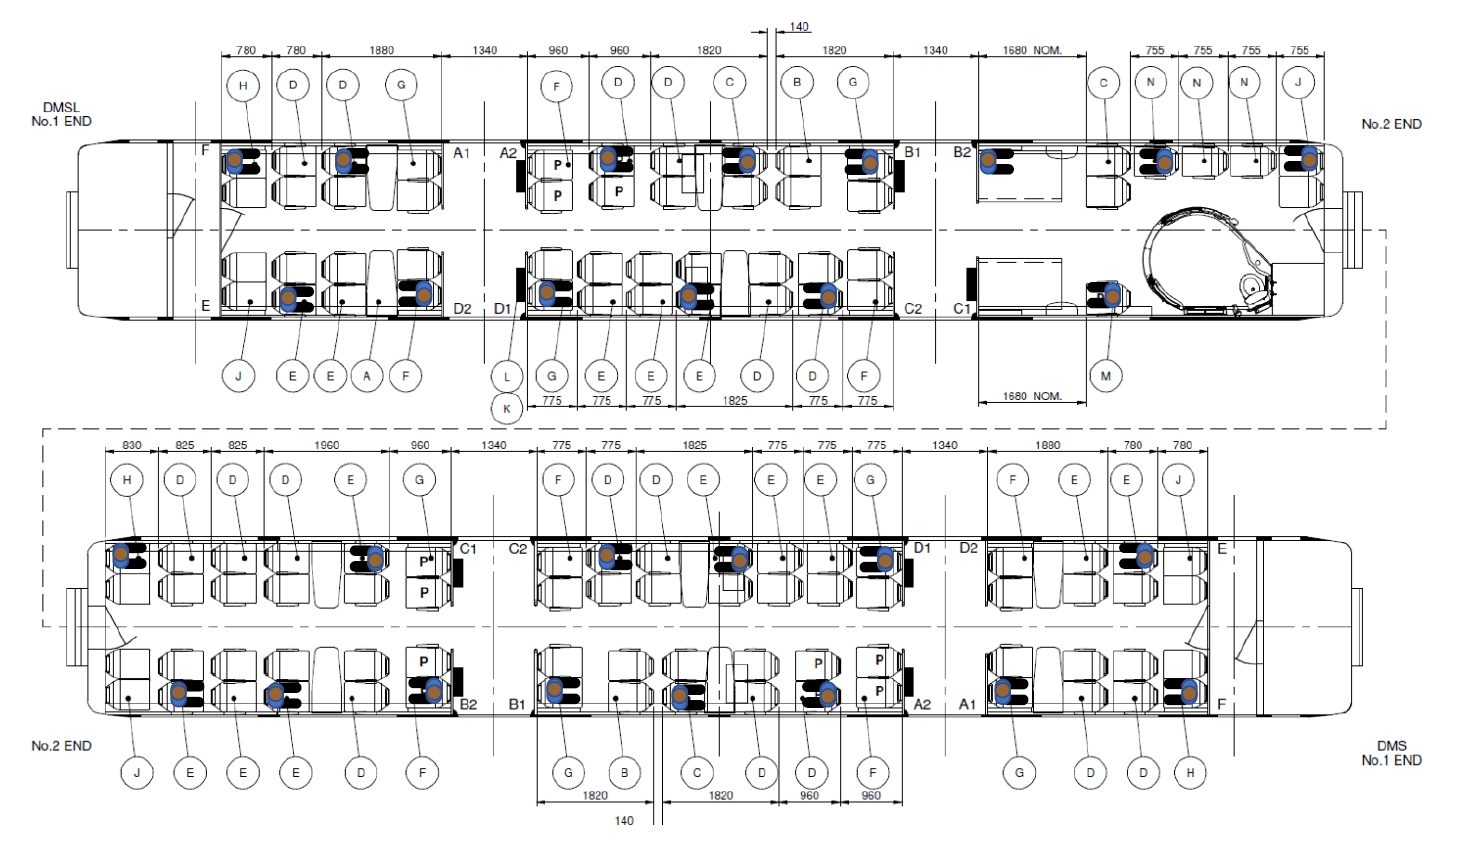
\includegraphics[scale = 0.6]{floorplan150.png}
\caption{The seating arrangement for the class 150 train.}
\label{Reference}
\end{subfigure}
~
\begin{subfigure}[h]{0.49\linewidth}
\centering
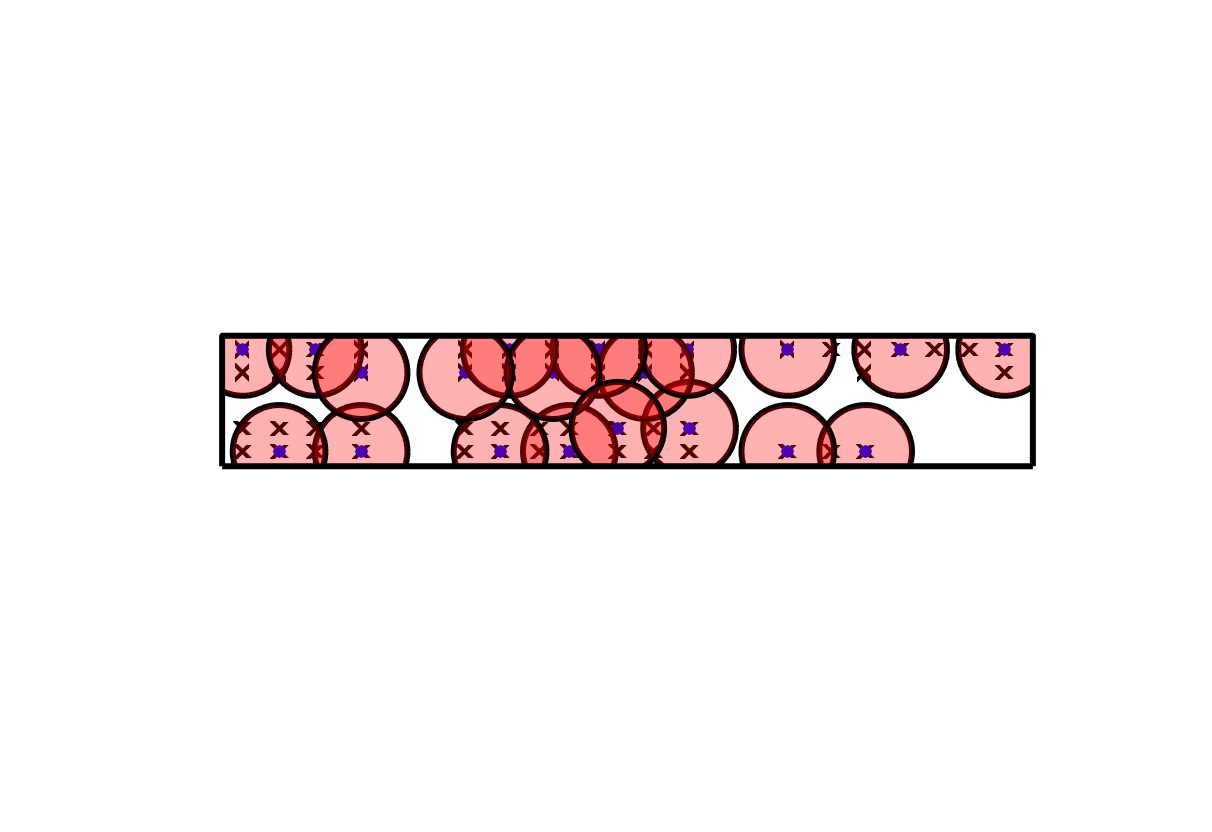
\includegraphics[width = \linewidth]{class150_first_car_1m.png}
\caption{A sample layout for carriage 1 with a social distancing measure of $1$ metres. $20$ seats are available.}
\label{OneMetre1}
\end{subfigure}
~
\begin{subfigure}[h]{0.490\linewidth}
\centering
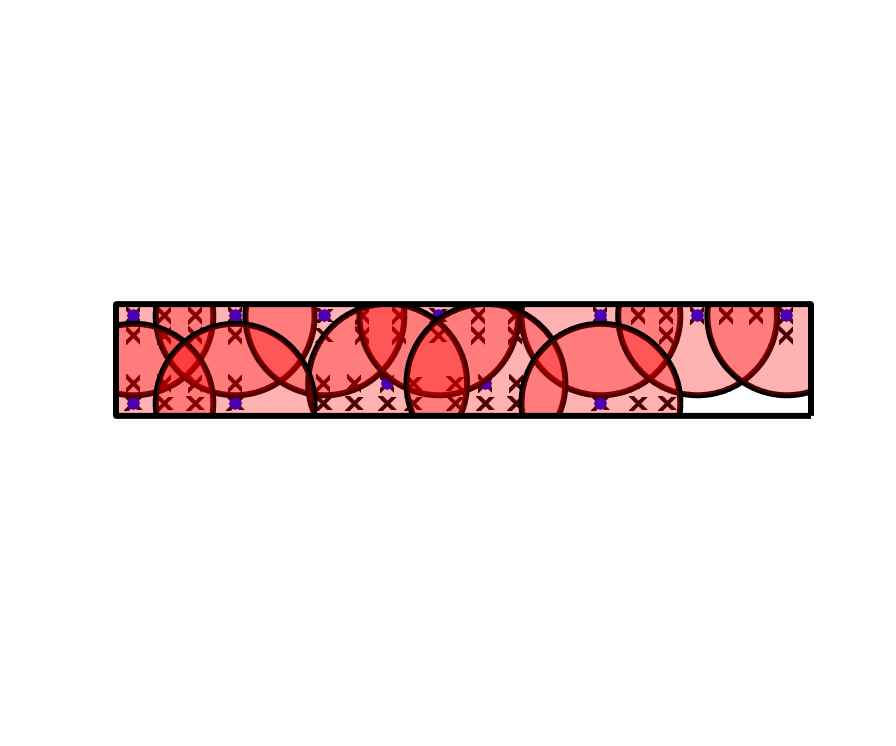
\includegraphics[width = \linewidth]{class150_first_car_2m.png}
\caption{A sample layout for carriage 1 with a social distancing measure of $2$ metres. $13$ seats are available.}
\label{TwoMetre1}
\end{subfigure}
~
\begin{subfigure}[h]{0.49\linewidth}
\centering
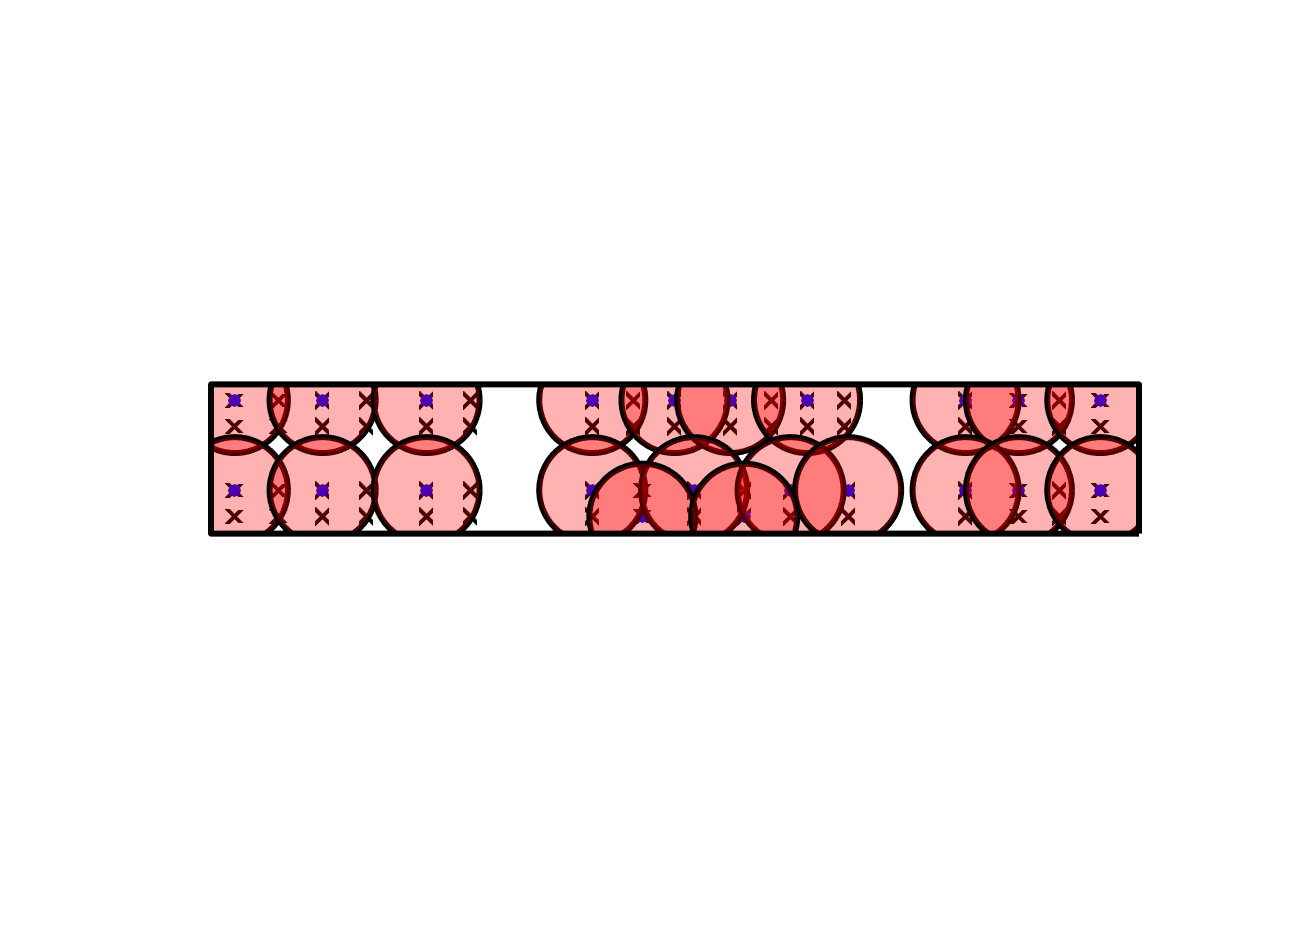
\includegraphics[width = \linewidth]{class150_second_car_1m.png}
\caption{A sample layout for carriage 2 with a social distancing measure of $1$ metres. $22$ seats are available.}
\label{OneMetre2}
\end{subfigure}
~
\begin{subfigure}[h]{0.490\linewidth}
\centering
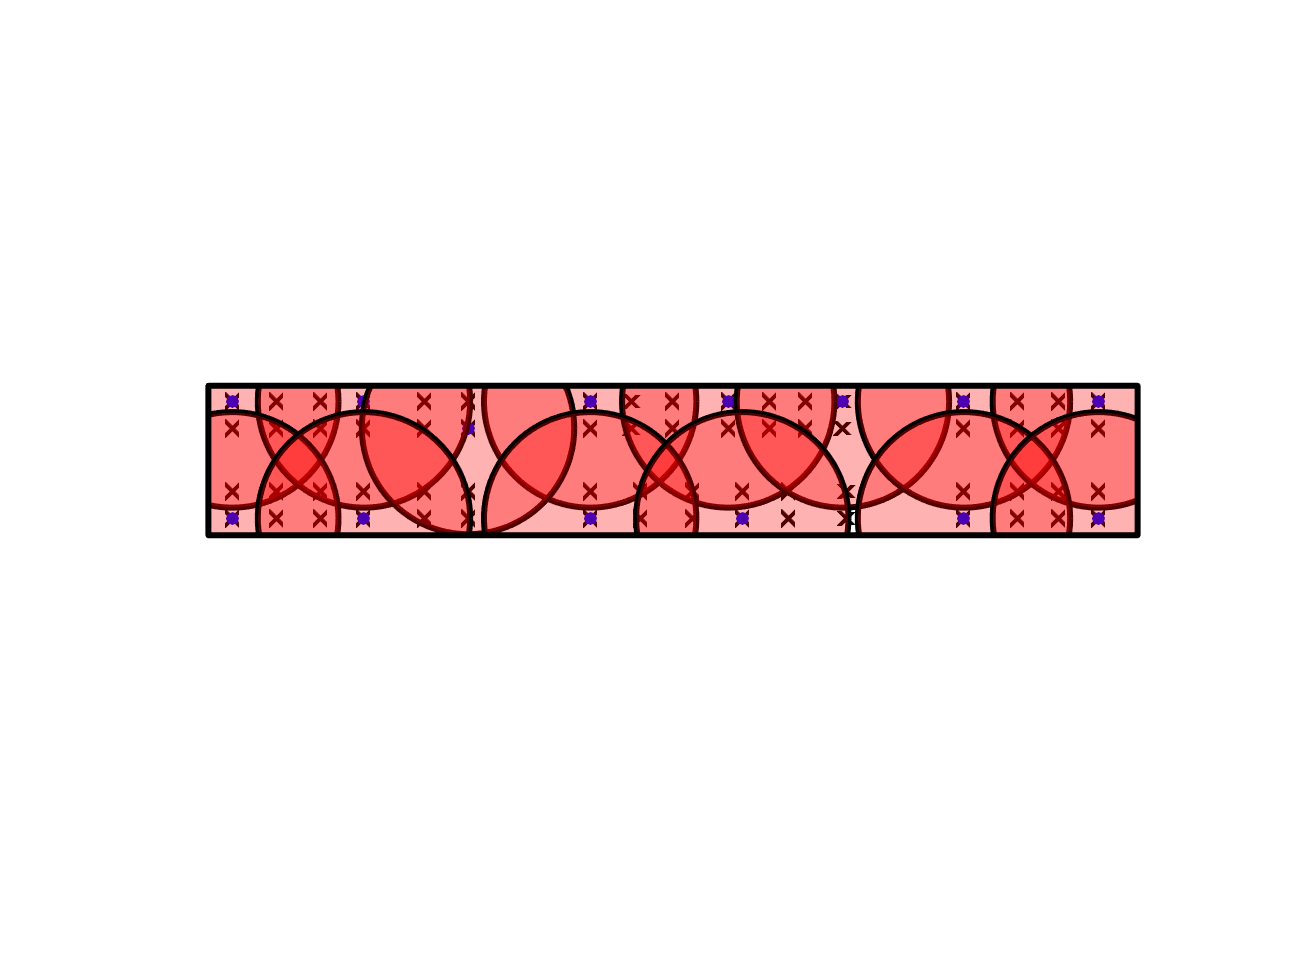
\includegraphics[width = \linewidth]{class150_second_car_2m.png}
\caption{A sample layout for carriage 2 with a social distancing measure of $2$ metres. $14$ seats are available.}
\label{TwoMetre2}
\end{subfigure}
\caption{A proposed seating layout given by the app for $1$ and $2$ metre social distancing for both carriages of the class 150 train. Seat locations are marked with crosses, available seats are marked with dots and the `region of safety' is denoted by a circle around the available seats. Overlapping circles imply that certain regions are exposed to contamination from multiple sources, but no available seats are located in these regions. }
\label{Demonstration_pics}
\end{figure*}


\begin{table}[ht!]
\begin{center}
 \begin{tabular}{|c |c|}
 \hline
& \textbf{Maximum capacity at $2$m social distancing }\\
 \hline
 Benchmark &   28 (23.3\%)\footnotemark \\
 \hline
 Cardiff App  & 27 (22.5\%)\\
\hline
\end{tabular}
\end{center}
\caption{Comparison of the performance of the Cardiff seat finding app against the benchmark provided in the supplied report.}
\label{tab:performance}
\end{table}


As demonstrated in Table \ref{tab:performance}, we can very quickly achieve similar occupancy rates in the train without violating social distancing measures. Given more time, we can develop methods for taking passenger direction into account, and geometrical constrains (walls/partitions in the carriages) allowing for higher occupancy rates.
\footnotetext{We note that in the provided estimation of the Class 150 design, there exists `usable' seats that are within 2 metres of each other.}

\section*{Prospective developments for improving optimality}
Our application always provides seating arrangements that obey social distancing measures, and provides locally optimal solutions which are similar the given benchmarks. Returning the  absolute optimum arrangement, however, is a lot more difficult because the problem is what is known as `NP-hard'.  Simply put, the only way to guarantee you have the most possible seats used is to try every possible order of seat checking, and pick the one which has the most seats used. Actually trying out every seat ordering would take a very long time; there are more ways to order $120$ seats than there are particles in the universe.\\

What we can do, though, is develop techniques to check our solutions and continuously improve upon them where possible. At a cost of additional time and computing power to implement, these methods would improve the likelihood we have found the best possible seating arrangement, allowing us to potentially further improve on our already powerful result. For example, we have a provided preliminary calculations in \autoref{fig:Stochastic_sims} to show that our current results are optimal up to 10,000 simulations, however, this can extended with computational power and theoretical applications.\\
\end{document}
